\documentclass{beamer}
\usetheme{AnnArbor}
\usecolortheme{spruce}
\usepackage{circuitikz}
\usepackage{graphicx}

\title{Adders, Encoders, and Decoders}
\subtitle{More sophisticated applications of circuits}
\author[A Praveen \& A Krishnan]{Akilesh Praveen \& Ashwath Krishnan}
\institute{UMD}
\date{\today}



\begin{document}

    % title page
    \begin{frame}
        \titlepage
    \end{frame}
    
    % table of contents
    \begin{frame}
        \frametitle{Agenda}
        \tableofcontents
    \end{frame}
    
    \section{Announcements}
    
        \begin{frame}
                \vfill
                \centering
                \begin{beamercolorbox}[sep=8pt,center,shadow=true,rounded=true]{title}
                    \usebeamerfont{title}Announcements\par%
                \end{beamercolorbox}
                \vfill
             \end{frame}
    
        \subsection{Project 2}
        
            
            
            \begin{frame}
                \frametitle{Project 2}
                \begin{itemize}
                    \item Project 2 has been released, and can be found on the course website under 'Week 3' on the calendar.
                    \item Everything you need to complete the project will be covered in today's lecture, with optional supplementary material provided on the course website under Week 3's resources section.
                    
                \end{itemize}
            \end{frame}
            
            \begin{frame}
            	\frametitle{Some Reminders}
            	\begin{itemize}
            		\item As the projects become more involved, we'd like to remind you to reach out and attend office hours if you are struggling.
                    \item Additionally, here's a reminder that all projects can be group projects, but you'll have to let us know \textbf{4 days} prior to the project's due date if you'll be working in a group. (Max size of 3)
            	\end{itemize}
            	
            \end{frame}
        
    \section{Adders}
    
    	\begin{frame}
                \vfill
                \centering
                \begin{beamercolorbox}[sep=8pt,center,shadow=true,rounded=true]{title}
                    \usebeamerfont{title}Adders\par%
                \end{beamercolorbox}
                \vfill
             \end{frame}
    
    	\subsection{Addition}
    
    	\begin{frame}
    		\frametitle{Addition}
    		\begin{center}
    			{\Large How would you add the following binary numbers?}
    			\linebreak
    			{\Large \texttt{11101} \& \texttt{11011}}
    		\end{center}
    	\end{frame}
    	
    	\begin{frame}
    		\frametitle{Addition}
    		\begin{itemize}
    			\item Let's visualize the computation as long addition
    			\item How would you go about solving it this way?
			\end{itemize}
			
			\centering
			{\LARGE
			\begin{tabular}{c@{\,}c@{\,}c@{\,}c@{\,}c@{\,}c@{\,}c}
					   & 1 & 1 & 1 & 0 & 1 \\
					 + & 1 & 1 & 0 & 1 & 1 \\
					\hline
					
			\end{tabular}}
		\end{frame}
		
		\begin{frame}
    		\frametitle{Addition}
    		\begin{itemize}
    			\item Let's visualize the computation as long addition
    			\item How would you go about solving it this way?
			\end{itemize}
			
			\centering
			{\LARGE
			\begin{tabular}{c@{\,}c@{\,}c@{\,}c@{\,}c@{\,}c@{\,}c}
					   &   &   &   & {\color{red}1} &   \\
					   & 1 & 1 & 1 & 0 & 1 \\
					 + & 1 & 1 & 0 & 1 & 1 \\
					\hline
					   &   &   &   &   & 0
					
			\end{tabular}}
			
			\begin{itemize}
				\item This phenomenon is known as a {\color{red}carry}
				\item This occurs when the numbers we are adding exceed the limit imposed by the number system we are using
				\item Where else during this computation would this phenomenon occur?
			\end{itemize}
		\end{frame}	
		
		\subsection{Half Adders}
		
		\begin{frame}
			\frametitle{Half Adders}
			\begin{itemize}
				\item First, let's represent the \texttt{1}s as \texttt{TRUE}s and the \texttt{0}s as \texttt{FALSE}s
				\item Think back to last week when we talked about designing circuits that dealt with booleans
				\item The big question: can we perform the addition process that we just talked about using such gates?
				\item The answer: \textbf{absolutely}
			\end{itemize}
		\end{frame}
		
		\begin{frame}
			\frametitle{Half Adders}
			\begin{itemize}
				\item Let's take this step by step.
				\item Looking at the addition example, what's the simplest operation we can take away from that?
				\item Let's see if we can build something that can take two one-bit numbers and add them, producing a carry if applicable
				\begin{itemize}
					\item In terms of inputs, we will need two booleans
					\item In terms of outputs, we will need two booleans (one for our sum, and one for the carry)
				\end{itemize}
				\item Incidentally, we have been describing a \textbf{Half Adder}
				\item We have defined our inputs and outputs- try to design a Half Adder using the gates we've learned
			\end{itemize}
			
				
		\end{frame}
		
		\begin{frame}
			\frametitle{Half Adders}
			\begin{itemize}
				\item Below is the formal truth table and circuit diagram for an optimal Half-Adder
				\item In this case, we can see that the Sum and Carry can be represented by an \texttt{XOR} and \texttt{AND} gate, respectively \linebreak
			\end{itemize}
			\centering
			\begin{columns}
				\column{0.5\textwidth}
					\centering
					\begin{tabular}{ |p{0.75cm}||p{0.75cm}||p{0.75cm}|}
                    	 \hline
                     	\multicolumn{3}{|c|}{Half Adder} \\
                     	\hline
                     	In & Sum & Carry\\
                     	\hline
                     	0 0 & 0 & 0\\
                     	0 1 & 1 & 0\\
                     	1 0 & 1 & 0\\
                     	1 1 & 0 & 1\\
                    	 \hline
                	\end{tabular}
				
				\column{0.5\textwidth}
					\centering
					
					% HALF ADDER
					
					\begin{circuitikz} \draw
                    (-1.5,2.22) node[](b) {B}
                    (-1.5,2.78) node[](a) {A}
                    
                    (1.5,2.5) node[xor port] (myxor) {}
                    (1.5,1) node[and port] (myand) {}
                    
                    (-0.25,2.78) node[circ] (circ1) {}
                    (-0.5,2.22) node[circ] (circ2) {}
                    
                    (2.25,2.5) node[] (S) {SUM}
                    (2.35, 1) node[] (C) {CARRY}
                    
                    
                    (a) -| (myxor.in 1) 
                    (a) -| (circ1) 
                    (b) -| (myxor.in 2)
                    (b) -| (circ2)
                    (-0.25,2.78) -- (-0.25,1.28) -- (0.25,1.28)
                    (-0.5,2.22) -- (-0.5,0.72) -- (0.25,0.72);
                    
                    \end{circuitikz}
				
				
			\end{columns}
		\end{frame}

		\subsection{Full Adders}	
		
		\begin{frame}
			\frametitle{Full Adders}
			\begin{itemize}
				\item The Half Adder is great, but limited in functionality
				\item Let's work on 'scaling' it for use with multi-digit addition.
				\item How do we accomplish such a task?
				\item All we need to do is create a circuit that can:
				\begin{itemize}
					\item Add two one-bit numbers and produce a sum and carry
					\item In case the previous addition resulted in a carry, be able to add in that third number as well
				\end{itemize}
				\item Essentially, we need a logical circuit that can add three one-bit numbers. We can then use this circuit for each digit in our addition.
			\end{itemize}
		\end{frame}
		
		\begin{frame}
			\frametitle{Full Adders}
			\begin{itemize}
				\item Below is a full adder that meets our previously outlined specifications exactly.
			\end{itemize}
			
			\centering
			\begin{circuitikz}
			\draw
			(3,0) node[xor port] (myxor) {} to
			(7,0) node[xor port,anchor=in 2] (myxor1) {}
			(0,-2) node[and port,rotate=270] (myand) {}
			(5,-2) node[and port,rotate=270] (myand1) {}
			
			(2.5,-4) node[or port,rotate=270] (myor) {}
			(myxor.in 1) -- +(-2.5,0) node[anchor=east] (a) {A}
			(myxor.in 2) -- +(-2.5,0) node[anchor=east] (b) {B}
			(myor.out) node[anchor=north] (co) {Carry out}
			(myxor.in 2 -| myand.in 1) node[circ] {} -- (myand.in 1)
			(myxor.in 1 -| myand.in 2) node[circ] {} -- (myand.in 2)
			(myand.out) |- (myor.in 2)
			(myand1.out) |- (myor.in 1)
		
			(myand1.in 1) -- +(0,1.5) node[anchor=south] (cin) {Carry in}
			(myand1.in 1 |- myxor1.in 1) node[circ] {} -- (myxor1.in 1)
			(myxor1.in 2 -| myand1.in 2) node[circ] {} -- (myand1.in 2)
			(myxor1.out) node[anchor=west] (sum) {Sum}
			;
			\end{circuitikz}
		\end{frame}
		
		\begin{frame}
			\frametitle{Full Adders}
			\begin{itemize}
				\item However, it's important to note that there's an easier way to think about the implementation of a full adder
				\item Notice that the Half Adder already has half the functionality of the Full Adder that we need to design
				\begin{itemize}
					\item Specifically, it can add two one-bit numbers and produce a sum and carry. All we need to add is the ability to carry a bit into the addition.
				\end{itemize}
				\item That being said, let's try and employ the use of Half Adders within our Full Adder construction
			\end{itemize}
		\end{frame}
		
		\begin{frame}
			\frametitle{Full Adders}
			\begin{itemize}
				\item Take a look at this Full Adder construction, built using Half Adders.
			\end{itemize}
			\centering
			\begin{circuitikz} \draw
			(0,1.5) node[] (a) {A}
			(0,0) node[] (b) {B}
			(0,-1.5) node[] (c) {$C_{in}$}
			(8.25,0) node[] (sum) {SUM}
			(10.35,-3.28) node[] (cout) {$C_{out}$}
			
			(2.25,0.75) node[] (ha1) {HA}
			(6.25,-0.75) node[] (ha2) {HA}

			(1.25, 1.75) -- (1.25, -0.25) -- (3.25, -0.25) -- (3.25, 1.75) -- (1.25, 1.75)
			
			(0.25, 1.5) -- (1.25, 1.5)
			(0.25, 0) -- (1.25, 0) 

			(3.25, 1.5) -- (4.5, 1.5)
			(4.5,1.5) -- (4.5,0)
			(4.5,0) -- (5.25,0)
			
			(5.25,0.25) -- (7.25,0.25) -- (7.25,-1.75) -- (5.25, -1.75) -- (5.25,0.25) 
				
			(3.25, 0) -- (4, 0)
			(4,0) -- (4,-3.56)
			(4,-3.56)--(8.5,-3.56)	
			(9.75,-3.28) node[or port] (myor) {}	
			
			(0.25, -1.5) -- (3.8, -1.5)
			(3.8, -1.5) -- (3.8, -1.3)
			(3.8, -1.3) -- (4.2, -1.3)
			(4.2, -1.3) -- (4.2, -1.5)
			(4.2, -1.5) -- (5.25, -1.5)
			
			(7.25,0) -- (7.75, 0)
			(7.25,-1.5) -- (8.4, -1.5)
			(8.4, -1.5) -- (8.4, -3)
			
			;
			\end{circuitikz}
		\end{frame}
		
		\begin{frame}
			\frametitle{Full Adders}
			\begin{itemize}
				\item If full adders are better than half adders, why do we use them?
				\item During addition of any size, you may notice that there is always one addition 'operation' that will never have a 'carry in'
				\begin{itemize}
					\item This will always occur in the least significant bit
				\end{itemize}
				\item Since a half adder is fundamentally simpler than a full adder, we always use it when we can
				\item Now that we have the ability to add two one bit numbers, with or without a carried '1' coming into the addition, let's put these together (literally) and create a multiple digit adder.
			\end{itemize}
		\end{frame}
		
		
		\begin{frame}
			\frametitle{Full Adders}
			\begin{itemize}
				\item Here's an example of how we can chain adders to increase the number of bits that we can perform addition with
				\item Note that the Full Adder handling \texttt{A0} and \texttt{B0} can be replaced with a Half Adder\linebreak
			\end{itemize}
			
			
			
			\centering
			
			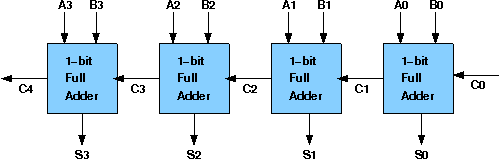
\includegraphics[width=0.8\textwidth]{4bitadder}
			
			\centering
			{\tiny Image courtesy of IIT}
			
		\end{frame}
		
		\begin{frame}
			\frametitle{Full Adders}
			
			\begin{itemize}
				\item Okay, now we can add simple n-bit numbers. But then how can computers show us numbers that aren't in binary?
				\item We need a way to translate these binary signals into numbers that we can use (or that a computer can display for us)
				\item In other words, we need to somehow convert the outputs to base-10
			\end{itemize}
			
		\end{frame}
		
		
    
    
\end{document}
